\documentclass[twoside]{article}
\usepackage[obeyspaces]{url}
\usepackage{natbib}
%\usepackage{chem}
\usepackage{color}
\usepackage{rotating} % loads graphicx
%\usepackage{longtable}
\usepackage{graphicx}
%\usepackage{verbatim}
%\usepackage{draftwatermark}\SetWatermarkScale{6}
\usepackage{ulem}
\usepackage{fancyvrb}
\usepackage{amssymb}
\usepackage[intlimits,fleqn,tbtags]{amsmath}

%\usepackage[nodayofweek]{datetime}
%\renewcommand{\dateseparator}{.}
%\newcommand{\todayiso}{\twodigit\day \dateseparator \twodigit\month \dateseparator \the\year}

% Chemistry
%\usepackage[version=3]{mhchem}
\usepackage[]{chem}

% Listings
\usepackage{listings}
\definecolor{gray}{gray}{.25}

\DeclareRobustCommand*\degree{\ensuremath{^{\circ}}}

\usepackage[nottoc]{tocbibind}
\settocbibname{References}          %%% Title of bibliography

\usepackage{hyperref}
\hypersetup{
%    bookmarks=true,         % show bookmarks bar?
  colorlinks=true,
  linkcolor=black,
  filecolor=black,
  urlcolor=black,
  citecolor=black,
  pdftex=true,
  plainpages=false,
  hypertexnames=true,
  pdfpagelabels=true,
  unicode=true,
  pdftoolbar=true,
  pdfmenubar=true,
  pdffitwindow=true,
  pdfcreator={TeX},
  pdfproducer={pdfTeX-1.40},
  pdfnewwindow=false
}

\oddsidemargin-5mm
\evensidemargin-15mm
\topmargin-15mm
\textheight240mm
\textwidth180mm
\raggedbottom
\parindent0mm
\parskip1.0ex plus0.5ex minus0.5ex
\renewcommand{\arraystretch}{1}
\renewcommand{\topfraction}{0.95}
\renewcommand{\dbltopfraction}{0.95}
\renewcommand{\bottomfraction}{0.95}
\renewcommand{\floatpagefraction}{0.95}
\renewcommand{\dblfloatpagefraction}{0.95}
\renewcommand{\textfraction}{0.01}
\setcounter{topnumber}{3}
\setcounter{secnumdepth}{4}
\setcounter{tocdepth}{4}

\newcommand{\egcite}[1]{\citep[e.g.][]{#1}}
\newcommand{\etccite}[1]{\citep[and references therein]{#1}}
\newcommand{\hhline}{\noalign{\vspace{1mm}}\hline\noalign{\vspace{1mm}}}
\newcommand{\hhlines}{\noalign{\vspace{1mm}}\hline\hline\noalign{\vspace{1mm}}}
\newcommand{\kpproot}{{\sc root}}
\newcommand{\todo}[1]{{\uppercase{\bf ((#1))}}}
\newcommand{\update}[1] {\textcolor{red}{#1}}

\def\mypageheader{B. Kern: SCALC User Manual}
\markboth{\mypageheader}{\mypageheader}
\pagestyle{myheadings}

\begin{document}

\thispagestyle{empty}
%\vspace*{-2cm}
\begin{center}
  {\Huge\bf SCALC User Manual}\\[3mm]
  {\huge\it for the Simple CALCulations submodel, version 1.7}\\[9mm]
  {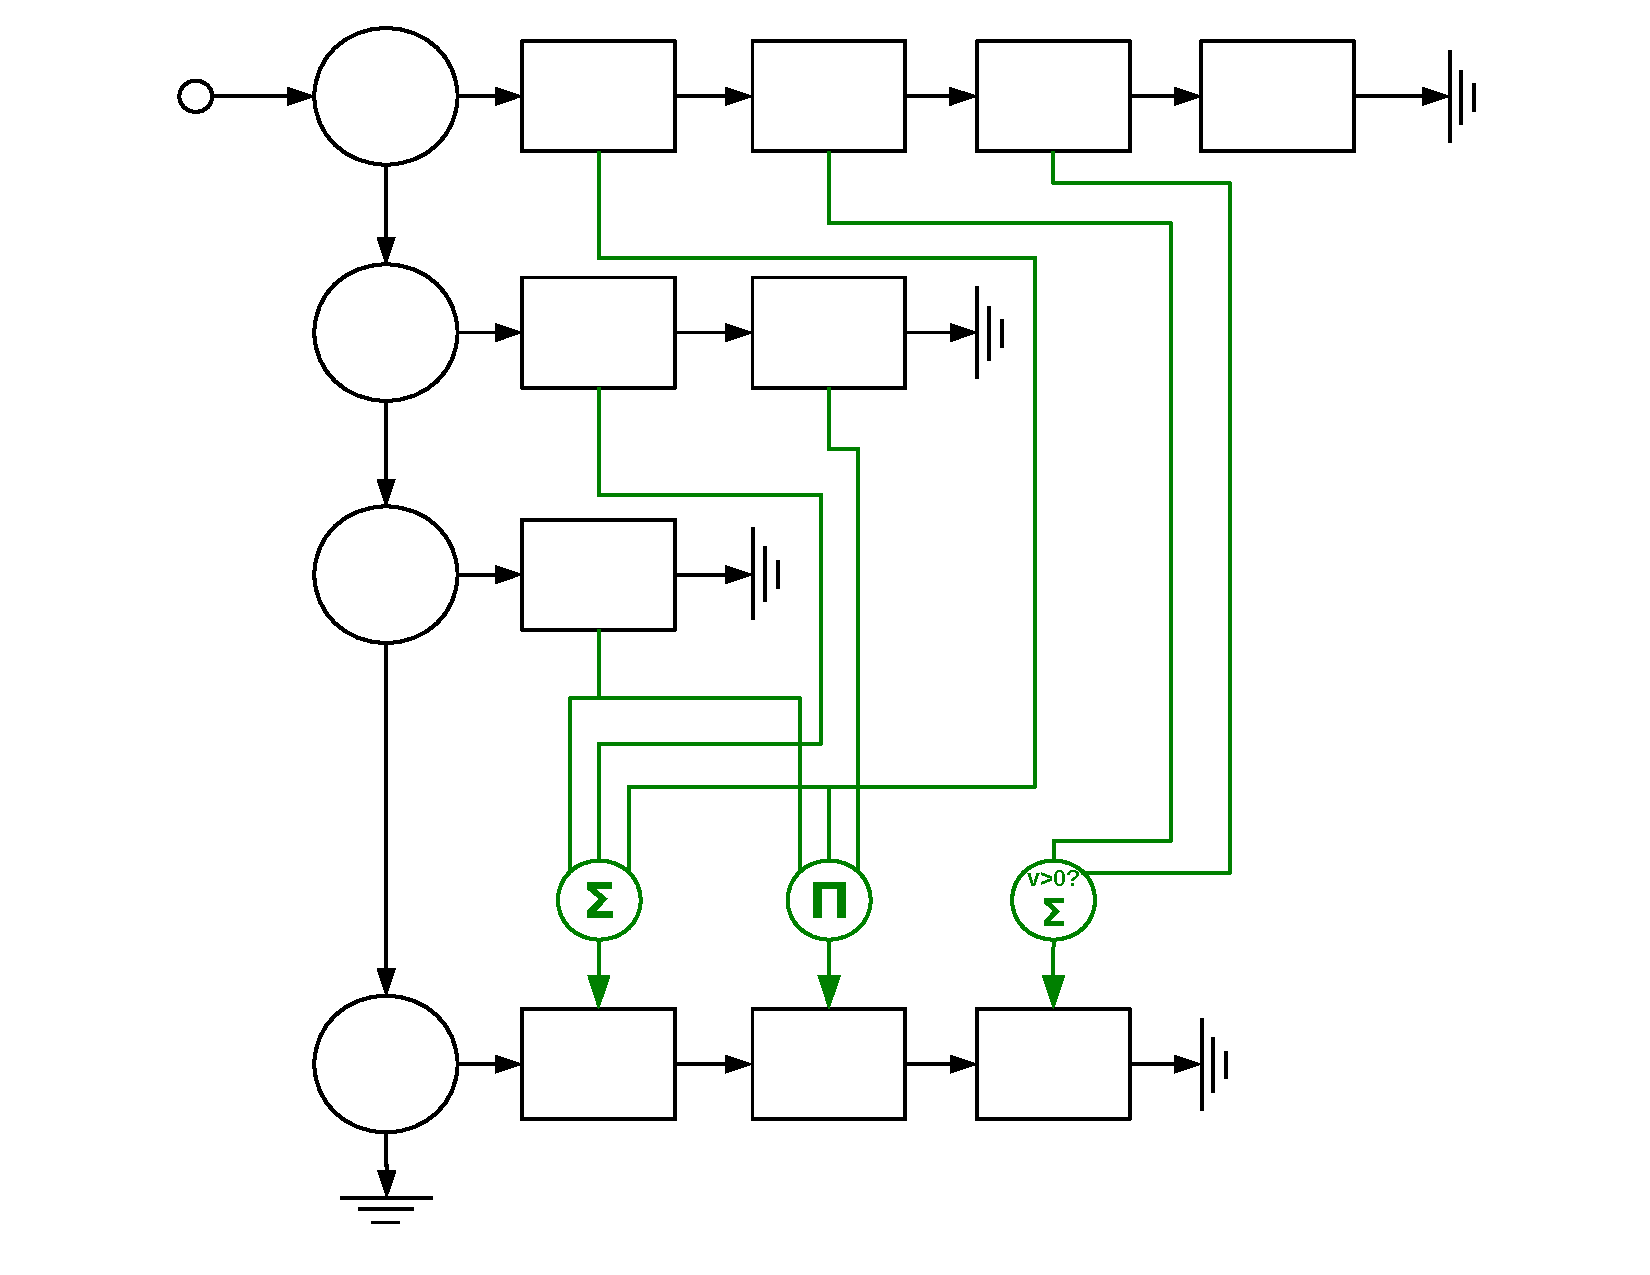
\includegraphics[width=0.7\textwidth]{scalc_front}}\\[21mm]
  {\LARGE\bf Bastian Kern}\\[9mm]
  \Large
  Deutsches Zentrum f\"{u}r Luft- und Raumfahrt, Institut
  f\"{u}r Physik der Atmosph\"{a}re, Oberpfaffenhofen, 82234 Wessling,
       Germany\\
  \url{bastian.kern@dlr.de}

\end{center}

\vfill

%{\large This manual is part of the electronic supplement of\\
%B. Kern and P. J\"{o}ckel, ``The Modular Earth Submodel System (MESSy, 2.50\_extended) as diagnostic interface of the ICOsahedral Non-hydrostatic (ICON) modelling framework'', Geosci.\ Model\ Dev.\ (2016), available at: \url{http://www.geoscientific-model-development.net}}

\begin{center}
%  Date: \thedate
  Date: \today
\end{center}

\newpage
\tableofcontents
\newpage
%%%%%%%%%%%%%%%%%%%%%%%%%%%%%%%%%%%%%%%%%%%%%%%%%%%%%%%%%%%%%%%%%%%%%%%%%%%%%%
%% ###########################################################################
%%%%%%%%%%%%%%%%%%%%%%%%%%%%%%%%%%%%%%%%%%%%%%%%%%%%%%%%%%%%%%%%%%%%%%%%%%%%%%
\section{Acknowledgement}
%%%%%%%%%%%%%%%%%%%%%%%%%%%%%%%%%%%%%%%%%%%%%%%%%%%%%%%%%%%%%%%%%%%%%%%%%%%%%%
%% ###########################################################################
%%%%%%%%%%%%%%%%%%%%%%%%%%%%%%%%%%%%%%%%%%%%%%%%%%%%%%%%%%%%%%%%%%%%%%%%%%%%%%
I thank all colleagues who contributed to the submodel by active development, bug reports and requests for additional functionality.
I'd like to thank Patrick, Mariano, Vanessa, Phoebe, and Duy for their developments and feedback.
I'm grateful to Vanessa and Mariano for their testing of SCALC version 1.0.
Thanks to Franziska for her development of {\tt DIV} and to Hiroshi for testing the {\tt QSUM} implementation.
Very special thanks to Astrid for her major developments, which lead to version 1.1 of SCALC.
%
%%%%%%%%%%%%%%%%%%%%%%%%%%%%%%%%%%%%%%%%%%%%%%%%%%%%%%%%%%%%%%%%%%%%%%%%%%%%%%
%% ###########################################################################
%%%%%%%%%%%%%%%%%%%%%%%%%%%%%%%%%%%%%%%%%%%%%%%%%%%%%%%%%%%%%%%%%%%%%%%%%%%%%%
\section{History}
%%%%%%%%%%%%%%%%%%%%%%%%%%%%%%%%%%%%%%%%%%%%%%%%%%%%%%%%%%%%%%%%%%%%%%%%%%%%%%
%% ###########################################################################
%%%%%%%%%%%%%%%%%%%%%%%%%%%%%%%%%%%%%%%%%%%%%%%%%%%%%%%%%%%%%%%%%%%%%%%%%%%%%%
\begin{table}[h!]
  \begin{tabular}{ l r r l l }
    Date       & SCALC & MESSy   & Developer          & Changes\\
    \hline
    08.07.2011 & v0.1 & 2.42     & Bastian Kern       & Initial implementation of SCALC, only SUM supported\\
    18.09.2015 & v0.1 &          & Mariano Mertens    & Extension of calculations: SUMGE0 \\
    02.03.2016 & v0.1 & 2.53.0   & Patrick J\"{o}ckel & Calculations at \texttt{global\_start}, \texttt{global\_end} or both\\
    21.04.2017 & v1.0 &          & Bastian Kern       & Enhanced error handling and namelist checking\\
               &      &          &                    & Extension of calculations: MULT, PSUM, PSUMDIA\\
               &      &          &                    & First version of user manual\\
    21.03.2018 & v1.0 & 2.54.0   & Franziska Frank    & Implementation of mathematical operator DIV\\
    27.03.2019 & v1.1 & 2f124e05 & Astrid Kerkweg     & Usage of 2D horizontal slices of 3D data objects\\
               &      &          &                    & Multiple analysis of CPL namelist \\
               &      &          &                    & Set entry points for calculation in namelist via strings\\
    28.03.2019 & v1.2 & 25e678aa & Bastian Kern       & Implementation of mathematical operator QSUM\\
    15.05.2019 & v1.2 &          & Bastian Kern       & User manual updates:\\
               &      &          &                    & DIV and QSUM, entry points, limitations\\
    May 2020   & v1.6 &          & Mariano Mertens    & FLAG, FLAGU, FLAGD operators\\
    18.06.2020 & v1.7 & f7c56131 & Patrick J\"{o}ckel & DELTA operator\\
    18.06.2020 & v1.8 & bbdabb91 & Patrick J\"{o}ckel & WVA operator\\
    Jan 2021   & v1.9 &          & Franziska Winterstein & SPLITV operator\\
    \hline
  \end{tabular}
   \caption{Overview of the developments in SCALC. Git commit IDs correspond to commits pushed to the MESSy development repository at {\tt https://gitlab.dkrz.de/MESSy/MESSy.git}.}
   \label{tab:versions}
\end{table}

Development of this submodel was initiated when I needed some special functionality.
This functionality was the summation of some model variables and the provision of the result as a new variable.
With the concept of CHANNEL in the MESSy (Modular Earth Submodel System; \citealt{Jockel2005,Jockel2010}) framework, this was straight forward to implement.

I used the first version of SCALC (which only supported this simple summation) during my PhD \citep{Kern2013} to calculate the total dust deposition flux from the partial fluxes, provided by DDEP (Dry DEPosition; \citealp{Kerkweg2006}), SEDI (SEDImentation; \citealp{Kerkweg2006}) and SCAV (SCAVenging; \citealp{Tost2006}).
The deposition fluxes in DDEP and SEDI consist of four different particle classes (soluble Aitken mode, insoluble Aitken mode, soluble coarse mode, insoluble coarse mode), in SCAV the coarse mode fluxes are partitioned in fluxes from large scale and convective precipitation.
All these fluxes were summed up and fed as new channel object into the submodel A2O (Atmosphere TO Ocean; \citealp{Pozzer2011}), which performs a grid transformation from the atmospheric grid to the oceanic grid.
In the ocean, the dust flux was used as input to the interactive oceanic biogeochemistry (HAMOCC, HAMburg Ocean Carbon Cycle Model; \citealp{Maier-Reimer2005, Wetzel2005, Kern2013}).

Years after that study some colleagues asked me how to use SCALC for their setups, and they asked if SCALC could be extended to multiplication and some kind of positive confined summation.
So, I started a new development cycle for SCALC, which is now available in version 1.0.
During extended tests, we found some bugs in the error handling.
This new version collects extensions in functionality as well as improved error handling and namelist checking.
I decided to use version 1.0 for this new extended and tested version of SCALC, to show that the submodel could be used (with appropriate caution) by all MESSy users.
Now, with more users applying SCALC and the extensions in the calculation options, there is a need for a user manual, which goes (a tiny bit) beyond the 1.25 pages available in Appendix C of \citet{Kern2013}.
This user manual gives an overview of the submodel and lists all available options of SCALC, which can be controlled via Fortran namelists.\\

Bastian Kern, 21.04.2017, SCALC v1.0\\

After some time, the user manual lacked behind the actual code of SCALC.
Some extensions were implemented and included in several versions of MESSy, an overview is given at the beginning of this user manual in Tab. \ref{tab:versions}.
This revision of the user manual contains the description of SCALC and its updates.

I thank Astrid for her major contributions to SCALC and the updates to this user manual.

I'm happy if you contact me in case you detect something weird and you think it might be a bug in SCALC, or you want to extend the submodel.\\

Bastian Kern, 15.05.2019, SCALC v1.2\\

%%%%%%%%%%%%%%%%%%%%%%%%%%%%%%%%%%%%%%%%%%%%%%%%%%%%%%%%%%%%%%%%%%%%%%%%%%%%%%
%% ###########################################################################
%%%%%%%%%%%%%%%%%%%%%%%%%%%%%%%%%%%%%%%%%%%%%%%%%%%%%%%%%%%%%%%%%%%%%%%%%%%%%%
\section{Introduction}
%%%%%%%%%%%%%%%%%%%%%%%%%%%%%%%%%%%%%%%%%%%%%%%%%%%%%%%%%%%%%%%%%%%%%%%%%%%%%%
%% ###########################################################################
%%%%%%%%%%%%%%%%%%%%%%%%%%%%%%%%%%%%%%%%%%%%%%%%%%%%%%%%%%%%%%%%%%%%%%%%%%%%%%
%
The Simple CALCulations (SCALC) submodel can be used to perform calculations on model variables and return the result in a new variable.
The submodel's calculations work on {\it channel objects} and provide their results as {\it channel objects} (see the CHANNEL user manual in the supplement of \citealp{Jockel2010}).
SCALC supports the calculation of sums (including some special kinds, explained below) products, and fractions.
For interoperability between SCALC and different MESSy submodels, the calculations can be performed basically everywhere within the time loop (the call just needs to be implemented in the CONTROL). This ensures, that a valid result is available to other submodels via the CHANNEL infrastructure.
All basemodels feature calculations at the beginning and/or the end of the model's time loop.
The user interface is implemented via Fortran namelists and follows the MESSy standard.
The user can control, which calculation is performed, on which {\it channel objects} and at which state of the model's time integration.
Consistency checks for the namelist options and error handling when accessing {\it channel objects} are performed.
Although, users should read this manual and carefully check their namelist setup when using this submodel, to avoid unwanted results.

%%%%%%%%%%%%%%%%%%%%%%%%%%%%%%%%%%%%%%%%%%%%%%%%%%%%%%%%%%%%%%%%%%%%%%%%%%%%%%
%% ###########################################################################
%%%%%%%%%%%%%%%%%%%%%%%%%%%%%%%%%%%%%%%%%%%%%%%%%%%%%%%%%%%%%%%%%%%%%%%%%%%%%%
\section{Limitations}
%%%%%%%%%%%%%%%%%%%%%%%%%%%%%%%%%%%%%%%%%%%%%%%%%%%%%%%%%%%%%%%%%%%%%%%%%%%%%%
%% ###########################################################################
%%%%%%%%%%%%%%%%%%%%%%%%%%%%%%%%%%%%%%%%%%%%%%%%%%%%%%%%%%%%%%%%%%%%%%%%%%%%%%
%
Version 1.2 of SCALC is not tested to work on multiple nested domains (patches).

It is possible to use SCALC {\it channel objects} as input in subsequent SCALC calculations, depending on the order of calls to SCALC.
Calls to SCALC are implemented at several points in the basemodel (as defined in CONTROL; cf. Sec. \ref{sec:contextstring}).
Before using a specific entry point, the user should check its availability.

The user is advised to check the results carefully!

%%%%%%%%%%%%%%%%%%%%%%%%%%%%%%%%%%%%%%%%%%%%%%%%%%%%%%%%%%%%%%%%%%%%%%%%%%%%%%
%% ###########################################################################
%%%%%%%%%%%%%%%%%%%%%%%%%%%%%%%%%%%%%%%%%%%%%%%%%%%%%%%%%%%%%%%%%%%%%%%%%%%%%%
\section{SCALC namelist user interface}
\label{sec:scalcui}
%%%%%%%%%%%%%%%%%%%%%%%%%%%%%%%%%%%%%%%%%%%%%%%%%%%%%%%%%%%%%%%%%%%%%%%%%%%%%%
%% ###########################################################################
%%%%%%%%%%%%%%%%%%%%%%%%%%%%%%%%%%%%%%%%%%%%%%%%%%%%%%%%%%%%%%%%%%%%%%%%%%%%%%
The user interface of SCALC is implemented via Fortran namelists provided in the {\tt scalc.nml} file.
Listing \ref{lst:scalc.nml} shows an example of the SCALC namelists.
According to the MESSy standard \citep{Jockel2005,Jockel2010}, the namelist file contains a {\tt CTRL} and a {\tt CPL} namelist.
At the moment, there are no namelist parameters in the {\tt CTRL} namelist for SCALC.
The {\tt CPL} namelist contains the actual setup for SCALC.
The user can provide different {\tt CALC} entries, which specify mathematical operations to be executed on user defined {\it channel objects} and which return the result of the specific operation as a new {\it channel object} in the {\tt scalc} {\it channel}.

\begin{lstlisting}[language=FORTRAN,
   breaklines=true, %
   basicstyle=\ttfamily,        % the size of the fonts that are used for the code
   breakatwhitespace=true,         % sets if automatic breaks should only happen at whitespace
   prebreak={\raisebox{0ex}[0ex][0ex]{\space\ensuremath{\boldsymbol{\hookleftarrow}}}},
   commentstyle=\color{gray},
   label={lst:scalc.nml},
   caption = {Example namelist {\tt scalc.nml} of the SCALC submodel. For explanations, see text.}
   ]
&CTRL
/
&CPL
! ### SYNTAX:
! # CALC(.) = 'object-name', 'list-of-channel-objects', 'operation',when?,
! # : when: string of entry point
! # : list of channel objects = 'ch1:obj1%s1,obj2%s2,...;cha2:obj1%s1,...;'
! # : s1, s1, ... optional scaling factors
! # : operation = SUM, PSUM, PSUMDIA, SUMGE0, QSUM, MULT, DIV, ...
!
CALC(1) = 'sum_out', 'channel1:object1,object2%2.0;channel2:object3', 'SUM', 'messy_global_start',
CALC(2) = 'psum_out', 'channel1:object1,object2%-1.0', 'PSUM', 'messy_global_end',
CALC(3) = 'psumdia_out', 'channel1:object1,object2%-1.0', 'PSUMDIA', 'messy_global_end',
CALC(4) = 'sumge0_out', 'channel1:object1;channel2:object4', 'SUMGE0', 'messy_global_start;messy_global_end,0',
CALC(5) = 'q_out', 'channel1:qv;channel2:H2O', 'QSUM', 'messy_global_end',
CALC(6) = 'vmr_out', 'channel2:H2O;channel1:qv', 'QSUM', 'messy_global_end',
CALC(7) = 'product_out', 'channel1:object5;channel2:object6', 'MULT', 'messy_global_end',
CALC(8) = 'division_out', 'channel1:object6;channel2:object7', 'DIV', 'messy_global_end',
!
/
\end{lstlisting}
%
%%%%%%%%%%%%%%%%%%%%%%%%%%%%%%%%%%%%%%%%%%%%%%%%%%%%%%%%%%%%%%%%%%%%%%%%%%%%%%
\subsection{The {\tt CALC} structure variable}
\label{sec:calcstructure}
%%%%%%%%%%%%%%%%%%%%%%%%%%%%%%%%%%%%%%%%%%%%%%%%%%%%%%%%%%%%%%%%%%%%%%%%%%%%%%
%
The user can specify different {\tt CALC} entries in {\tt scalc.nml}, the numbering of these has to be unique.
In the current implementation, a maximum of {\tt NMAXCALC = 100} {\tt CALC} entries is allowed (see Listing \ref{lst:CALC} in Sec. \ref{sec:implementationcalcstructure}).

The {\tt CALC} structure variable contains four strings:

The first string names the result of the operation, this name is used for naming the {\it channel object} and has to be unique for the {\tt scalc} {\it channel}.

The second string is the channel object string, which defines all {\it channel objects} involved in the operation. The channel object string is composed according to the rules in Section \ref{sec:objectstring}.

The third string defines which mathematical operation is applied by SCALC to the defined objects.
Valid choices are {\tt SUM}, {\tt PSUM}, {\tt PSUMDIA}, {\tt SUMGE0}, {\tt
  QSUM}, {\tt MULT}, {\tt DIV}, {\tt FLAG}, {\tt FLAGU}, {\tt FLAGD}, {\tt
  DELTA}($R_{std}$,$n$), {\tt WVA}, and {\tt SPLITV}.
Definitions of the operations can be found in Section \ref{sec:operations}.

The last string defines in which context (entry point) the mathematical operation has to be executed by SCALC.
Details to the context string can be found in Section \ref{sec:contextstring}.

For further explanation on the concept of {\it channels} and {\it channel objects} from MESSy CHANNEL see \citet{Jockel2010}.
%
%%%%%%%%%%%%%%%%%%%%%%%%%%%%%%%%%%%%%%%%%%%%%%%%%%%%%%%%%%%%%%%%%%%%%%%%%%%%%%
\subsection{Channel object string}
\label{sec:objectstring}
%%%%%%%%%%%%%%%%%%%%%%%%%%%%%%%%%%%%%%%%%%%%%%%%%%%%%%%%%%%%%%%%%%%%%%%%%%%%%%
%
SCALC works on two- and three-dimensional {\it channel objects}.
Generally, all objects have to be of the same {\it representation}.
However, combinations of two-dimensional {\it channel objects} on representations {\tt GP\_2D\_HORIZONTAL} and {\tt GP\_3D\_1LEV} are allowed, the resulting {\it channel object} has the {\it representation} of the first {\it channel object} in the channel object string specified in the {\tt CPL} namelist.
Since the version 1.1, two-dimensional horizontal slices of three-dimensional {\it channel objects} are possible (see below).
In this case, the resulting {\it channel objects} need to be of the same representation.

The channel object string contains all {\it channel objects} and optional scaling factors, which will be combined in the new {\it channel object} in {\it channel} {\tt scalc}, which name is specified within the first string of the {\tt CALC} variable.

In the second string ({\tt str}) the user has to specify all {\it channel objects} for the operation according to the following syntax:

\begin{lstlisting}[breaklines=true, %
   basicstyle=\ttfamily,        % the size of the fonts that are used for the code
   breakatwhitespace=true,         % sets if automatic breaks should only happen at whitespace
   prebreak={\raisebox{0ex}[0ex][0ex]{\space\ensuremath{\boldsymbol{\hookleftarrow}}}},
   ]
<channel>:<object>[\%<scal>\&<lev>][,<object>[\%<scal>\&<lev>]][,...] [;<channel>:<object>[\%<scal>]\&<lev>[,...]][;...]
\end{lstlisting}

{\it Channel objects} have to be specified by their {\it channel name} and {\it object name} separated by colon.
If there are more {\it objects} from one {\it channel}, they can be separated by comma without specifying the {\it channel name} again.
Separation of {\it channel objects} from different {\it channels} is by semicolon.
Optional constant scaling factors can be provided for each {\it channel object} individually by appending it to the {\it object name} separated by a percentage sign.
In addition, three-dimensional {\it channel objects} can be reduced to horizontal two-dimensional slices by indicating the respective level index preceded by an ampersand. {\tt <lev>} can either be a number or the identifier {\tt LL} indicating the lowest model layer.

Note that {\tt LL} is always replaced by the number of vertical model levels (e.g. {\tt nlev}).
Even for {\it channel objects} which are defined on interface levels, {\tt nlev} and not {\tt nlev+1} is used if {\tt LL}  is specified.
%
%%%%%%%%%%%%%%%%%%%%%%%%%%%%%%%%%%%%%%%%%%%%%%%%%%%%%%%%%%%%%%%%%%%%%%%%%%%%%%
\subsection{Context string}
\label{sec:contextstring}
%%%%%%%%%%%%%%%%%%%%%%%%%%%%%%%%%%%%%%%%%%%%%%%%%%%%%%%%%%%%%%%%%%%%%%%%%%%%%%
%
The string consists of entry point names, defined in {\tt messy\_main\_control.f90}, and an optional integer, denoting the trigger location in the entry point.
The string has the form:

{\tt <entry point>[,<location>][;<entry point>[,<location>]][;...]}

The defined entry points are:

\begin{tabular}{l@{\hspace{4em}}l@{\hspace{4em}}l@{\hspace{4em}}l}
   {\tt messy\_setup}         & {\tt messy\_initialize}    & {\tt messy\_new\_tracer}    & {\tt messy\_tracer\_meta}    \\
   {\tt messy\_init\_memory}  & {\tt messy\_init\_coupler} & {\tt messy\_init\_coupling} & {\tt messy\_read\_restart}   \\
   {\tt messy\_init\_tracer}  & {\tt messy\_init\_loop}    & {\tt messy\_time}           & {\tt messy\_tendency\_reset} \\
   {\tt messy\_global\_start} & {\tt messy\_local\_start}  & {\tt messy\_beforeadv}      & {\tt messy\_afteradv}        \\
   {\tt messy\_radiation}     & {\tt messy\_vdiff}         & {\tt messy\_radheat}        & {\tt messy\_gwdrag}          \\
   {\tt messy\_convec}        & {\tt messy\_mixlo}         & {\tt messy\_physc}          & {\tt messy\_local\_end}      \\
   {\tt messy\_global\_end}   & {\tt messy\_write\_output} & {\tt messy\_write\_restart} & {\tt messy\_free\_memory}    \\
   {\tt messy\_finalize}      &                            &                             &                              \\
\end{tabular}

Note that calls to SCALC during the time loop are implemented exactly where they are required for diagnostics.
The first SCALC implementation (v1.0) just required calls in the entry points {\tt messy\_global\_start} and  {\tt messy\_global\_end}.
However, in the course of the implementation of model coupling strategies, calls to SCALC at very precise points during the time loop became necessary.
Thus, calls to SCALC are implemented everywhere where they are required currently.
In future, additional calls can be easily added to the CONTROL file.

For one coupling SCALC needs to be called at least twice from different places in one entry point, to pre- and post-process data before and after the coupling, respectively.
Therefore the {\tt location} integers have been introduced as handles to discriminate SCALC calls within the same entry point.
%
%%%%%%%%%%%%%%%%%%%%%%%%%%%%%%%%%%%%%%%%%%%%%%%%%%%%%%%%%%%%%%%%%%%%%%%%%%%%%%
%% ###########################################################################
%%%%%%%%%%%%%%%%%%%%%%%%%%%%%%%%%%%%%%%%%%%%%%%%%%%%%%%%%%%%%%%%%%%%%%%%%%%%%%
\section{Operations}
\label{sec:operations}
%%%%%%%%%%%%%%%%%%%%%%%%%%%%%%%%%%%%%%%%%%%%%%%%%%%%%%%%%%%%%%%%%%%%%%%%%%%%%%
%% ###########################################################################
%%%%%%%%%%%%%%%%%%%%%%%%%%%%%%%%%%%%%%%%%%%%%%%%%%%%%%%%%%%%%%%%%%%%%%%%%%%%%%
%
Several options for mathematical operations are implemented.
\begin{itemize}
   \item{\tt SUM} Summation of all channel objects in the channel object string
   \item{\tt PSUM} Positive confined summation
   \item{\tt PSUMDIA} Positive confined summation, combined with an error diagnostic
   \item{\tt SUMGE0} Summation of two channel objects in case the value of the first object is lower or equal a tiny number ($1\cdot10^{-20}$)
   \item{\tt QSUM} Summation of water tracer channel objects of different units
   \item{\tt MULT} Product of all channel objects
   \item{\tt DIV} Division operator
   \item{\tt FLAG} Multiplication (flagging) of a 2D/3D field with a 2D field containing 0/1
   \item{\tt FLAGD} As FLAG, but all values lower than 0.99 in the provided flag field are set to 0 ('flagdown')
   \item{\tt FLAGU} As FLAG, but all values larger than 0.01 in the provided flag field are set to 1  ('flagup')
   \item{\tt DELTA}($R_{std}$,$n$) Calculation of the fractions of rare and
     abundant isotopologue from the isotopic signature ($\delta$-value in
     permil).
   \item{\tt WVA} Calculation of the weighted vertical average
   \item{\tt SPLITV}($s$) Split 3D field vertically into two along 2D field with
     level indices ($s$ selects the oprator for comparison)
\end{itemize}

%%%%%%%%%%%%%%%%%%%%%%%%%%%%%%%%%%%%%%%%%%%%%%%%%%%%%%%%%%%%%%%%%%%%%%%%%%%%%%
\subsection{Summation ({\tt SUM})}
\label{sec:summation}
%%%%%%%%%%%%%%%%%%%%%%%%%%%%%%%%%%%%%%%%%%%%%%%%%%%%%%%%%%%%%%%%%%%%%%%%%%%%%%
%
This option returns the sum over all {\it channel objects} specified in the channel object string via the Fortran {\tt CPL} namelist.
The result $\Phi$ at the location described by the indices $i$, $j$ and $k$ is the sum over all values $\phi_l$ of the defined channel objects $l=1,..,L$ at the same location.
The optional scaling factor $s_l$ for object $l$ has the value defined in the Fortran {\tt CPL} namelist or is equal to $1$, if it is not given for the respective object.
%
\begin{equation}
\Phi(i,j,k) = \sum_{l=1}^Ls_l\,\phi_l(i,j,k)
\end{equation}
%
%%%%%%%%%%%%%%%%%%%%%%%%%%%%%%%%%%%%%%%%%%%%%%%%%%%%%%%%%%%%%%%%%%%%%%%%%%%%%%
\subsection{Positive confined summation ({\tt PSUM}, {\tt PSUMDIA})}
\label{sec:positive_summation}
%%%%%%%%%%%%%%%%%%%%%%%%%%%%%%%%%%%%%%%%%%%%%%%%%%%%%%%%%%%%%%%%%%%%%%%%%%%%%%
%
{\tt PSUM} and {\tt PSUMDIA} return the same value as {\tt SUM}, if the calculated value is greater than $0$.
Otherwise the return value is set to 0.
In this way the result is confined to positive values.
%
\begin{equation}
\Phi(i,j,k) =
\begin{cases}
  \sum_{l=1}^Ls_l\,\phi_l(i,j,k), &\text{if } \sum_{l=1}^Ls_l\,\phi_l(i,j,k) > 0\\
  0,                             &\text{otherwise}
\end{cases}\\
\end{equation}
%
When using {\tt PSUMDIA} an additional diagnostic of the error produced by setting negative values to $0$ is stored in the {\it channel} {\tt scalc\_diag}.
The object name in {\tt scalc\_diag} is the object name given in {\tt CALC} appended by the string ``\_err''.
The value $\Phi_{\text{err}}$ is calculated as:
%
\begin{equation}
\Phi_{\text{err}}(i,j,k) =
\begin{cases}
  0,                                    &\text{if } \sum_{l=1}^Ls_l\,\phi_l(i,j,k) > 0\\
  \sum_{l=1}^Ls_l\,\phi_l(i,j,k), &\text{otherwise}
\end{cases}
\end{equation}
%
%%%%%%%%%%%%%%%%%%%%%%%%%%%%%%%%%%%%%%%%%%%%%%%%%%%%%%%%%%%%%%%%%%%%%%%%%%%%%%
\subsection{Summation greater equal zero ({\tt SUMGE0})}
\label{sec:summation_ge0}
%%%%%%%%%%%%%%%%%%%%%%%%%%%%%%%%%%%%%%%%%%%%%%%%%%%%%%%%%%%%%%%%%%%%%%%%%%%%%%
%
The name of the operation {\tt SUMGE0} is a bit misleading.
This operation calculates the sum over exactly two channel objects on a given location $(i,j,k)$ if the value of the first channel object on that location is less or equal a tiny number ($1\cdot10^{-20}$).
Otherwise the resulting value is set to $0$.
%
\begin{equation}
\Phi(i,j,k) =
\begin{cases}
  0,                        &\text{if } \phi_1(i,j,k) > 1\cdot10^{-20}\\
  \sum_{l=1}^2s_l\,\phi_l(i,j,k), &\text{otherwise}
\end{cases}\\
\end{equation}
%
This operation can only be used with exactly two {\it channel objects} in the channel object string, otherwise an error message is shown and the model execution is aborted.
%
%%%%%%%%%%%%%%%%%%%%%%%%%%%%%%%%%%%%%%%%%%%%%%%%%%%%%%%%%%%%%%%%%%%%%%%%%%%%%%
\subsection{Summation of water tracers ({\tt QSUM})}
\label{sec:summation_qsum}
%%%%%%%%%%%%%%%%%%%%%%%%%%%%%%%%%%%%%%%%%%%%%%%%%%%%%%%%%%%%%%%%%%%%%%%%%%%%%%
%
The summation of different water tracers is not straight forward if one or more tracers are given in the units of specific humidity, i.e. kg(\chem{H2O})/kg(moist air).
For summation of water tracers, all tracers have to be converted into units of mol(\chem{H2O})/mol(dry air), summed up, and (optionally) converted back in kg(\chem{H2O})/kg(moist air).
The units of the resulting field of this operation are determined by the units of the first input field.
Internally, the summation is conducted on fields with units mol(\chem{H2O})/mol(dry air).
The operation is evaluated as described in Section \ref{sec:summation} for {\tt SUM}.

If the units of the first channel object are "kg/kg" or "kg kg-1" a conversion to kg(\chem{H2O})/kg(moist air) is done at a last step in the summation operation.
Otherwise the result is not converted back and the units of the output channel are mol(\chem{H2O})/mol(dry air).
The resulting field's unit attribute is set to the same value as the value of the unit attribute of the first channel object.

Conversion of the water tracer field from specific humidity $q$ in kg(\chem{H2O})/kg(moist air) to volume mixing ratio $v_{\chem{H2O}}$ in mol(\chem{H2O})/mol(dry air) is:
\begin{equation}
   v_{\chem{H2O}} = \frac{\text{M}_{\text{air}}}{\text{M}_{\text{\chem{H2O}}}} \frac{q}{1 - q}
\end{equation}

Conversion of the water tracer field from volume mixing ratio $v_{\chem{H2O}}$ in mol(\chem{H2O})/mol(dry air) to specific humidity in kg(\chem{H2O})/kg(moist air) is:
\begin{equation}
   q = \frac{v_{\chem{H2O}}}{\frac{\text{M}_{\text{air}}}{\text{M}_{\text{\chem{H2O}}}} + v_{\chem{H2O}}}
\end{equation}

The quotient of molar mass of dry air $\text{M}_{\text{air}}$ and molar mass of water $\text{M}_{\text{\chem{H2O}}}$ is constant and evaluates to:
\begin{equation}
   \frac{\text{M}_{\text{air}}}{\text{M}_{\text{\chem{H2O}}}} = \frac{18.02\,\frac{\text{g}}{\text{mol}}}{28.97\,\frac{\text{g}}{\text{mol}}} \approx 0.622
\end{equation}
%
%
%%%%%%%%%%%%%%%%%%%%%%%%%%%%%%%%%%%%%%%%%%%%%%%%%%%%%%%%%%%%%%%%%%%%%%%%%%%%%%
\subsection{Multiplication ({\tt MULT})}
\label{sec:multiplication}
%%%%%%%%%%%%%%%%%%%%%%%%%%%%%%%%%%%%%%%%%%%%%%%%%%%%%%%%%%%%%%%%%%%%%%%%%%%%%%
This option returns the product over all {\it channel objects} specified in the channel object string via the Fortran {\tt CPL} namelist.
The result $\Phi$ at the location described by the indices $i$, $j$ and $k$ is the product over all values $\phi_l$ of the defined channel objects $l=1,..,L$ at the same location.
The optional scaling factor $s_l$ for object $l$ has the value defined in the Fortran namelist or is equal to $1$, if it is not given for the respective object.
%
\begin{equation}
\Phi(i,j,k) = \prod_{l=1}^Ls_l\,\phi_l(i,j,k)
\end{equation}
%
%
%%%%%%%%%%%%%%%%%%%%%%%%%%%%%%%%%%%%%%%%%%%%%%%%%%%%%%%%%%%%%%%%%%%%%%%%%%%%%%
\subsection{Division ({\tt DIV})}
\label{sec:division}
%%%%%%%%%%%%%%%%%%%%%%%%%%%%%%%%%%%%%%%%%%%%%%%%%%%%%%%%%%%%%%%%%%%%%%%%%%%%%%
This operator divides the first {\it channel object} by all following {\it channel objects} specified in the channel object string via the Fortran {\tt CPL} namelist.
The result $\Phi$ at the location described by the indices $i$, $j$ and $k$ is the quotient of value $\phi_1$ of the first channel object and all values $\phi_l$ of the subsequent defined channel objects $l=2,..,L$ at the same location.
The optional scaling factor $s_m$ for object $m$ ($m=1,..,L$) has the value defined in the Fortran namelist or is equal to $1$, if it is not given for the respective object.
%
\begin{equation}
   \Phi(i,j,k) = s_1\,\phi_1(i,j,k)\,\prod_{l=2}^L\,\frac{1}{s_l\,\phi_l(i,j,k)}
\end{equation}
%

%%%%%%%%%%%%%%%%%%%%%%%%%%%%%%%%%%%%%%%%%%%%%%%%%%%%%%%%%%%%%%%%%%%%%%%%%%%%%%
\subsection{Flagging ({\tt FLAG} {\tt FLAGD} {\tt FLAGU})}
\label{sec:flagging}
%%%%%%%%%%%%%%%%%%%%%%%%%%%%%%%%%%%%%%%%%%%%%%%%%%%%%%%%%%%%%%%%%%%%%%%%%%%%%%
This operator flags (i.e. multiplies) the first {\it channel object} with the second {\it channel object}, as defined in the {\tt CPL} namelist. The operator supports only two {\it channel objects}. If more {\it channel objects} are given in the {\tt CPL} namelist {\tt SCALC} will quit with an error message.
The first {\it channel object} can be a 2D or 3D field, the first two dimensions need to be latitude/longitude, the third dimension can  either be Z or N ({\it GP\_3D,GP\_2D,NX2D}).  The second {\it channel object} has to be 2D (lat/lon, {\it GP\_2D\_HORIZONTAL}). It should contain only values between 0-1 (this is not checked!).
Mathematically, the operators are a multiplication of the first and the second
{\it channel objects}. In the case that the first {\it channel objects} has
three dimensions, each hyperslab along the third dimensions is multiplied with the second {\it channel object}.  \\

The operators {\tt FLAGD} and {\tt FLAGU} are special cases of the {\tt FLAG} operator. They are introduced to circumvent problems, which can occur during the regridding of the 0-1 field (second {\it channel object}). When, for example, specific countries/continents should be flagged, and a (fine resolved) flag field is gridded onto a coarse grid, values between 0-1 will occur along the boundaries due to the regridding. This can lead to unwanted effects.
Therefore, the {\tt FLAGU} operator sets explicitely all values of the second {\it channel object} which are larger than 0.01 to 1 before the two {\it channel objects} are multiplied.
Similarly, the {\tt FLAGD} operator sets first all values of the second {\it channel object} which are lower than 0.99 to 0 before the multiplication.  \\

As an example for the usage of these two operators consider the case that
emissions should be split up in two regions: Europe and Rest of the World
(ROW).  With the {\tt FLAG} operator it can happen, that emissions along the
border lines of Europe are partly mapped to ROW instead of Europe. Therefore, the emissions of Europe are flagged with the {\tt FLAGU} operator and emissions from ROW with the {\tt FLAGD} operator.

%%%%%%%%%%%%%%%%%%%%%%%%%%%%%%%%%%%%%%%%%%%%%%%%%%%%%%%%%%%%%%%%%%%%%%%%%%%%%%
\subsection{Conversion of isotopic signature to fractions ({\tt DELTA}($R_{std}$,$n$))}
\label{sec:delta}
%%%%%%%%%%%%%%%%%%%%%%%%%%%%%%%%%%%%%%%%%%%%%%%%%%%%%%%%%%%%%%%%%%%%%%%%%%%%%%
This operator calculates the corresponding
fractions of the rare (minor) and abundant (major) isotopologe from the
$\delta$-value (in permil). The operator requires
one {\it channel object} containing the $\delta$-values, and
2 arguments:
$R_{std}$ is the ratio of the applied
standard (e.g. VSMOW or VPDB) and $n$ is the number of atoms of that
specific isotope in the molecule (e.g., n=1 for ${\delta}^{13}C(CH_4)$, n=4
for ${\delta}D(CH_4)$, etc.).

The isotopic ratio is calculated according to
%
\begin{equation}
   R = R_{std}  (\frac{\delta}{1000} + 1)
\end{equation}
and from those the fractions $f_r$ of the rare (major) and $f_{a}$ of the
abundant (minor) isotopoluge:
\begin{equation}
   f_{r} = \frac{n R}{1+R}; f_{a} = 1 - f_{r}
\end{equation}

The resulting {\it channel object} names are suffixed by {\tt \_01} for $f_r$,
and by {\tt \_02} for $f_a$ , respectively.

%%%%%%%%%%%%%%%%%%%%%%%%%%%%%%%%%%%%%%%%%%%%%%%%%%%%%%%%%%%%%%%%%%%%%%%%%%%%%%
\subsection{Calculation of the weighted vertical average ({\tt WVA})}
\label{sec:wva}
%%%%%%%%%%%%%%%%%%%%%%%%%%%%%%%%%%%%%%%%%%%%%%%%%%%%%%%%%%%%%%%%%%%%%%%%%%%%%%
This operator calculates the weighted vertical average. It requires two
3-dimensional {\it channel object}s, the first contains the data ($x$) to be
vertically averaged, the scond one contains the weight ($w$). The result is
a 2-dimensional {\it channel object} with the weigthed average ($\bar{x}$):
\begin{equation}
  \bar{x}(i,j) = \frac{\sum_{k=1}^{n_z}\,x(i,j,k)\,w(i,j,k)}
                      {\sum_{k=1}^{n_z}\,w(i,j,k)}~~.
\end{equation}

%%%%%%%%%%%%%%%%%%%%%%%%%%%%%%%%%%%%%%%%%%%%%%%%%%%%%%%%%%%%%%%%%%%%%%%%%%%%%%
\subsection{Split 3D field vertically along 2D filed with level indices ({\tt SPLITV}($s$))}
\label{sec:splitv}
%%%%%%%%%%%%%%%%%%%%%%%%%%%%%%%%%%%%%%%%%%%%%%%%%%%%%%%%%%%%%%%%%%%%%%%%%%%%%%
This operator splits a three dimensional {\it channel object} $o$ in gridpoint
representation into two {\it channel objects} $r_{01}$ and $r_{02}$ of the
same representation along a two dimensional {\it channel object} $h$
(horizontal) with level indices.
%
It requires as first entry the 3-dimensional {\it channel object} to be split,
and as second entry the 2-dimensional {\it channel object} with the
level indices. Furthermore, the operator takes one optional argument $s$ to
select the split operator: 0 for $\le$ (default) or 1 for $<$.
The result is two three dimensional {\it channel objects} suffixed
by {\tt \_01} and {\tt \_02}:
%
\begin{equation}
  r_{01}(i,j,k) =
\begin{cases}
  o(i,j,k) &\text{if } k \le h(i,j) \text{ and }  s = 0\\
  o(i,j,k) &\text{if } k < h(i,j)   \text{ and }  s = 1\\
  0        &\text{otherwise}
\end{cases}\\
\end{equation}

\begin{equation}
  r_{02}(i,j,k) =
\begin{cases}
  0         &\text{if } k \le h(i,j) \text{ and }  s = 0\\
  0         &\text{if } k < h(i,j)   \text{ and }  s = 1\\
  o(i,j,k)  &\text{otherwise}
\end{cases}\\
\end{equation}

%%%%%%%%%%%%%%%%%%%%%%%%%%%%%%%%%%%%%%%%%%%%%%%%%%%%%%%%%%%%%%%%%%%%%%%%%%%%%%
%% ###########################################################################
%%%%%%%%%%%%%%%%%%%%%%%%%%%%%%%%%%%%%%%%%%%%%%%%%%%%%%%%%%%%%%%%%%%%%%%%%%%%%%
\section{Implementation details}
%%%%%%%%%%%%%%%%%%%%%%%%%%%%%%%%%%%%%%%%%%%%%%%%%%%%%%%%%%%%%%%%%%%%%%%%%%%%%%
%% ###########################################################################
%%%%%%%%%%%%%%%%%%%%%%%%%%%%%%%%%%%%%%%%%%%%%%%%%%%%%%%%%%%%%%%%%%%%%%%%%%%%%%
%
The implementation of the SCALC submodel consists of {\tt smil/messy\_scalc\_si.f90} and {\tt smcl/messy\_scalc.f90}.
The following parameter definitions and subroutines are implemented in the submodel interface layer (SMIL).
Due to the internal implementation of the CHANNEL infrastructure, variable output for SCALC {\it channel objects} to files may lag one model time step behind.
The user should make sure, to use the correct position for the calculation of objects in the time loop, depending on which other submodels make use of the  SCALC {\it channel objects}.
The subroutine calls to the SCALC calculations are the first of all submodels for calculation in {\tt messy\_global\_start} and the almost last in {\tt messy\_global\_end}.
Submodel calls following {\tt scalc\_global\_end} are {\tt clams*\_global\_end}, {\tt vaxtra\_global\_end}, {\tt main\_tracer\_global\_end}, {\tt main\_tendency\_global\_end}, and {\tt main\_qtimer\_global\_end}.
A more precise method for calls to SCALC was introduced in version 1.1, details can be found in Sec. \ref{sec:contextstring}.
%
%%%%%%%%%%%%%%%%%%%%%%%%%%%%%%%%%%%%%%%%%%%%%%%%%%%%%%%%%%%%%%%%%%%%%%%%%%%%%%
\subsection{Mathematical operations}
\label{sec:mathoperations}
%%%%%%%%%%%%%%%%%%%%%%%%%%%%%%%%%%%%%%%%%%%%%%%%%%%%%%%%%%%%%%%%%%%%%%%%%%%%%%
%
Mathematical operations are defined through integer parameters.
During the calculation step a {\tt SELECT CASE} construct testing against these parameters selects the appropriate calculations.
%
\begin{verbatim}
  INTEGER, PARAMETER              :: SUM     = 1
  INTEGER, PARAMETER              :: PSUM    = 2
  INTEGER, PARAMETER              :: PSUMDIA = 3
  INTEGER, PARAMETER              :: SUMGE0  = 4
  INTEGER, PARAMETER              :: MULT    = 5
  INTEGER, PARAMETER              :: DIV     = 6
  INTEGER, PARAMETER              :: QSUM    = 7
  INTEGER, PARAMETER              :: FLAG    = 8
  INTEGER, PARAMETER              :: FLAGU   = 9
  INTEGER, PARAMETER              :: FLAGD   = 10
  INTEGER, PARAMETER              :: DELTA   = 11
  INTEGER, PARAMETER              :: WVA     = 12
  INTEGER, PARAMETER              :: SPLITV  = 13
\end{verbatim}
%
%%%%%%%%%%%%%%%%%%%%%%%%%%%%%%%%%%%%%%%%%%%%%%%%%%%%%%%%%%%%%%%%%%%%%%%%%%%%%%
\subsection{{\tt CALC} structure variable}
\label{sec:implementationcalcstructure}
%%%%%%%%%%%%%%%%%%%%%%%%%%%%%%%%%%%%%%%%%%%%%%%%%%%%%%%%%%%%%%%%%%%%%%%%%%%%%%
%
\begin{lstlisting}[language=FORTRAN,
   breaklines=true, %
   basicstyle=\ttfamily,        % the size of the fonts that are used for the code
   breakatwhitespace=false,         % sets if automatic breaks should only happen at whitespace
   prebreak={\raisebox{0ex}[0ex][0ex]{\space\ensuremath{\boldsymbol{\hookleftarrow}}}},
   commentstyle=\color{gray},
   label={lst:CALC},
   caption = {Definition of the structure variable {\tt CALC}. ({\tt smil/messy\_scalc\_si.f90})}
   ]
TYPE T_CALC_IO
   CHARACTER(LEN=STRLEN_OBJECT) :: object_name = ''  ! object to store result
   CHARACTER(LEN=STRLEN)        :: str = ''          ! channel/object string
   CHARACTER(LEN=8)             :: math_func_str = ''! math. funct. to use
   CHARACTER(LEN=STRLEN_ULONG)  :: when = 'messy_global_end'
END TYPE T_CALC_IO

TYPE T_CALC_CPL
   CHARACTER(LEN=STRLEN_OBJECT)   :: object_name = ''  ! object to store result
   CHARACTER(LEN=STRLEN)          :: str = ''          ! channel/object string
   CHARACTER(LEN=8)               :: math_func_str = ''! math. funct. to use
   INTEGER                        :: nwhen = 0
   INTEGER, DIMENSION(:), POINTER :: when  => NULL()
   INTEGER, DIMENSION(:), POINTER :: where => NULL()
END TYPE T_CALC_CPL

[...]

INTEGER, PARAMETER                           :: NMAXCALC = 100
TYPE(T_CALC_IO), DIMENSION(NMAXCALC),   SAVE :: CALC ! CPL namelist
\end{lstlisting}
The user defines the mathematical operations and the involved {\it channel objects} in the Fortran {\tt CPL} namelist in {\tt scalc.nml}.
A maximum of {\tt NMAXCALC} {\tt CALC} entries can be defined.
A description of the {\tt CALC} structure variable from a user's point-of-view is described in Section \ref{sec:calcstructure}.
%
%%%%%%%%%%%%%%%%%%%%%%%%%%%%%%%%%%%%%%%%%%%%%%%%%%%%%%%%%%%%%%%%%%%%%%%%%%%%%%
\subsection{Internal representation of calculation objects ({\tt XCALC})}
\label{sec:internalrepresentationcalc}
%%%%%%%%%%%%%%%%%%%%%%%%%%%%%%%%%%%%%%%%%%%%%%%%%%%%%%%%%%%%%%%%%%%%%%%%%%%%%%
%
The user defined {\tt CALC} entries from the {\tt CPL} namelist are converted into an internal representation.
For each user defined combination of {\it channel objects} and mathematical operation, an internal {\tt XCALC} variable is constructed.
The {\tt XCALC} structure contains the total number of objects ({\tt nobj}), lists of the extracted {\it channels} and {\it channel objects} ({\tt cha}, {\tt obj}), pointers to the actual data fields ({\tt dat2d}, {\tt dat3d}), the {\it representations} ({\tt rid}), and the physical units ({\tt unit}) for each {\it channel object}.
Furthermore the structure contains a pointer to the fields containing the result of the calculation ({\tt result2d}, {\tt result3d}) and to a field for diagnostic output ({\tt diag}).
Which input and output data fields to use ({\tt *2d} or {\tt *3d}) is determined by {\tt rank} of the {\tt channel objects}.
%
\begin{lstlisting}[language=FORTRAN,
   breaklines=true, %
   basicstyle=\ttfamily,        % the size of the fonts that are used for the code
   breakatwhitespace=false,         % sets if automatic breaks should only happen at whitespace
   prebreak={\raisebox{0ex}[0ex][0ex]{\space\ensuremath{\boldsymbol{\hookleftarrow}}}},
   commentstyle=\color{gray},
   label={lst:XCALC},
   caption = {Definition of the structure variable {\tt CALC}. ({\tt smil/messy\_scalc\_si.f90})}
   ]
TYPE T_CALC
   TYPE(T_CALC_CPL)             :: io
   ! number of objects in namelist
   INTEGER                      :: nobjnml
   ! number of objects after wildcard match
   INTEGER                      :: nobj
   LOGICAL                      :: ok
   INTEGER                      :: math_func         ! math. funct. to use
   CHARACTER(LEN=STRLEN_CHANNEL), DIMENSION(:), POINTER :: cha      => NULL()
   CHARACTER(LEN=STRLEN_OBJECT),  DIMENSION(:), POINTER :: obj      => NULL()
   REAL(DP),                      DIMENSION(:), POINTER :: tmp_fac  => NULL()
   LOGICAL,                       DIMENSION(:), POINTER :: lex      => NULL()
   ! POINTER TO DATA
   TYPE(PTR_2D_ARRAY),            DIMENSION(:), POINTER :: dat2d    => NULL()
   TYPE(PTR_3D_ARRAY),            DIMENSION(:), POINTER :: dat3d    => NULL()
   ! rank of data
   INTEGER,                       DIMENSION(:), POINTER :: rank     => NULL()
   ! REPRESENTATION ID
   INTEGER,                       DIMENSION(:), POINTER :: rid      => NULL()
   REAL(DP),                      DIMENSION(:), POINTER :: fac      => NULL()
   INTEGER,                       DIMENSION(:), POINTER :: tmp_lev  => NULL()
   INTEGER,                       DIMENSION(:), POINTER :: lev      => NULL()
   ! number of resulting channel objects
   INTEGER                                              :: nres      = 1
   ! number of operator parameters
   INTEGER                                              :: nparam    = 0
   REAL(DP),                      DIMENSION(:), POINTER :: xparam    => NULL()
   TYPE(PTR_2D_ARRAY),            DIMENSION(:), POINTER :: result2d  => NULL()
   TYPE(PTR_3D_ARRAY),            DIMENSION(:), POINTER :: result3d  => NULL()
   ! pointer to 2nd data array for diagnostic purposes
   TYPE(PTR_3D_ARRAY),                          POINTER :: diag     => NULL()
   ! unit string
   CHARACTER(LEN=STRLEN_ULONG), DIMENSION(:),   POINTER :: unit     => NULL()
END TYPE T_CALC

[...]

TYPE(T_CALC),    DIMENSION(:), POINTER, SAVE :: XCALC => NULL()
INTEGER,                                SAVE :: NCALC
\end{lstlisting}
%
%%%%%%%%%%%%%%%%%%%%%%%%%%%%%%%%%%%%%%%%%%%%%%%%%%%%%%%%%%%%%%%%%%%%%%%%%%%%%%
\subsection{{\tt scalc\_initialize}}
\label{sec:scalc_initialize}
%%%%%%%%%%%%%%%%%%%%%%%%%%%%%%%%%%%%%%%%%%%%%%%%%%%%%%%%%%%%%%%%%%%%%%%%%%%%%%
%
In this subroutine, the user defined {\tt CALC} entries from the {\tt CPL} namelist in {\tt scalc.nml} are read by calling the subroutine {\tt scalc\_read\_nml\_cpl}.
For each {\tt CALC} entry, the {\tt channel object} string and the string containing the entry points are parsed (subroutines {\tt str2chobfac} and {\tt parse\_when}, respectively)
and the individual {\tt XCALC} components  are constructed accordingly (see Listing \ref{lst:XCALC}).
Furthermore, the total number of requested calculations ({\tt NCALC}) is counted and some consistency checks are performed on the {\tt CALC} components.
%
%%%%%%%%%%%%%%%%%%%%%%%%%%%%%%%%%%%%%%%%%%%%%%%%%%%%%%%%%%%%%%%%%%%%%%%%%%%%%%
\subsection{{\tt scalc\_init\_memory(l\_cont)}}
\label{sec:scalc_init_memory}
%%%%%%%%%%%%%%%%%%%%%%%%%%%%%%%%%%%%%%%%%%%%%%%%%%%%%%%%%%%%%%%%%%%%%%%%%%%%%%
%
\begin{verbatim}
    LOGICAL, INTENT(IN), OPTIONAL :: flag
\end{verbatim}
This is a wrapper routine called from CONTROL in the entry point {\tt messy\_init\_memory}.
Its only objective is to call subroutine {\tt scalc\_init\_coupling(l\_cont)}.
It is, until now, only called in {\tt messy\_main\_control\_echam5.inc} for the ECHAM5 basemodel.
%
%%%%%%%%%%%%%%%%%%%%%%%%%%%%%%%%%%%%%%%%%%%%%%%%%%%%%%%%%%%%%%%%%%%%%%%%%%%%%%
\subsection{{\tt scalc\_init\_coupler(l\_cont)}}
\label{sec:scalc_init_coupler}
%%%%%%%%%%%%%%%%%%%%%%%%%%%%%%%%%%%%%%%%%%%%%%%%%%%%%%%%%%%%%%%%%%%%%%%%%%%%%%
%
\begin{verbatim}
    LOGICAL, INTENT(IN), OPTIONAL :: flag
\end{verbatim}
This is a wrapper routine called from CONTROL in the entry point {\tt messy\_init\_coupler}.
Its only objective is to call subroutine {\tt scalc\_init\_coupling(l\_cont)}.
Until now, it is only used in {\tt messy\_main\_control\_cosmo.inc} for the COSMO basemodel.
%
%%%%%%%%%%%%%%%%%%%%%%%%%%%%%%%%%%%%%%%%%%%%%%%%%%%%%%%%%%%%%%%%%%%%%%%%%%%%%%
\subsection{{\tt scalc\_init\_coupling(l\_cont)}}
\label{sec:scalc_init_coupling}
%%%%%%%%%%%%%%%%%%%%%%%%%%%%%%%%%%%%%%%%%%%%%%%%%%%%%%%%%%%%%%%%%%%%%%%%%%%%%%
%
\begin{verbatim}
    LOGICAL, INTENT(IN), OPTIONAL :: flag
\end{verbatim}
This subroutine creates the {\tt scalc} {\it channel} and (if needed) the {\tt scalc\_diag} {\it channel}.
It loops through all requested {\it channel objects} extracted from the user defined channel object string and tries to set pointers to the {\it channel object} data.
Additionally, the data components of the {\tt XCALC} structure variable are allocated.
If a request to a {\it channel object} fails, the model stops with an error message as long as {\tt l\_cont} is not set {\tt .TRUE.}.
When the subroutine is called with the optional parameter set {\tt l\_cont = .TRUE.}, the model will not stop and only produces a warning message in the log file, if a requested {\tt channel object} does not exists.
This is useful, if the subroutine is called several times, which is so far only required for model setups with OASIS coupling.
However, the last call needs to be with {\tt l\_cont=.FALSE.} otherwise, it might be, that inconsistent setups, where not all {\tt channel objects} could be associated, crash during runtime without meaning full error message.
For details on calling sequence/location of the SCALC subroutines, consult the {\tt messy\_main\_control\_*.inc} files.
%
%%%%%%%%%%%%%%%%%%%%%%%%%%%%%%%%%%%%%%%%%%%%%%%%%%%%%%%%%%%%%%%%%%%%%%%%%%%%%%
\subsection{{\tt scalc\_global\_start}}
\label{sec:scalc_global_start}
%%%%%%%%%%%%%%%%%%%%%%%%%%%%%%%%%%%%%%%%%%%%%%%%%%%%%%%%%%%%%%%%%%%%%%%%%%%%%%
%
This subroutine is called at the beginning of the model's time loop.
It calls the subroutine {\tt scalc\_integrate} to perform calculations, which should be executed at the beginning of the time loop (user controlled via {\tt CPL} namelist).
%
%%%%%%%%%%%%%%%%%%%%%%%%%%%%%%%%%%%%%%%%%%%%%%%%%%%%%%%%%%%%%%%%%%%%%%%%%%%%%%
\subsection{{\tt scalc\_convec}}
\label{sec:scalc_convec}
%%%%%%%%%%%%%%%%%%%%%%%%%%%%%%%%%%%%%%%%%%%%%%%%%%%%%%%%%%%%%%%%%%%%%%%%%%%%%%
%
This subroutine is called at the end of the model's time loop.
It calls the subroutine {\tt scalc\_integrate} to perform calculations, which should be executed in {\tt messy\_convec} (user controlled via {\tt CPL} namelist).
%
%%%%%%%%%%%%%%%%%%%%%%%%%%%%%%%%%%%%%%%%%%%%%%%%%%%%%%%%%%%%%%%%%%%%%%%%%%%%%%
\subsection{{\tt scalc\_physc}}
\label{sec:scalc_physc}
%%%%%%%%%%%%%%%%%%%%%%%%%%%%%%%%%%%%%%%%%%%%%%%%%%%%%%%%%%%%%%%%%%%%%%%%%%%%%%
%
This subroutine is called at the end of the model's time loop.
It calls the subroutine {\tt scalc\_integrate} to perform calculations, which should be executed in {\tt messy\_physc} (user controlled via {\tt CPL} namelist).
%
%%%%%%%%%%%%%%%%%%%%%%%%%%%%%%%%%%%%%%%%%%%%%%%%%%%%%%%%%%%%%%%%%%%%%%%%%%%%%%
\subsection{{\tt scalc\_global\_end}}
\label{sec:scalc_global_end}
%%%%%%%%%%%%%%%%%%%%%%%%%%%%%%%%%%%%%%%%%%%%%%%%%%%%%%%%%%%%%%%%%%%%%%%%%%%%%%
%
This subroutine is called at the end of the model's time loop.
It calls the subroutine {\tt scalc\_integrate} to perform calculations, which should be executed at the end of the time loop (user controlled via {\tt CPL} namelist).
%
%%%%%%%%%%%%%%%%%%%%%%%%%%%%%%%%%%%%%%%%%%%%%%%%%%%%%%%%%%%%%%%%%%%%%%%%%%%%%%
\subsection{{\tt scalc\_integrate}}
\label{sec:scalc_integrate}
%%%%%%%%%%%%%%%%%%%%%%%%%%%%%%%%%%%%%%%%%%%%%%%%%%%%%%%%%%%%%%%%%%%%%%%%%%%%%%
%
This subroutine executes the calculation for each {\tt XCALC} entry and stores the results in the {\tt XCALC} structure components {\tt result2d}/{\tt result3d}.
The calculation are performed, depending on the current context from which the subroutine is called (cf. Sec. \ref{sec:contextstring}).
The context is set in {\tt messy\_main\_control\_*.inc} indicating from which entry point messy subroutines have been called.
Thus it can be tested if the current position agrees with the user defined positions in the {\tt XCALC} entry (controlled via {\tt CPL} namelist).
Internally the context is evaluated by calling {\tt main\_control\_is\_context} with arguments {\tt when} and {\tt where} from the {\tt T\_CALC\_CPL} type (in structure {\tt XCALC\%io}).
%
%%%%%%%%%%%%%%%%%%%%%%%%%%%%%%%%%%%%%%%%%%%%%%%%%%%%%%%%%%%%%%%%%%%%%%%%%%%%%%
\subsection{{\tt scalc\_free\_memory}}
\label{sec:scalc_free_memory}
%%%%%%%%%%%%%%%%%%%%%%%%%%%%%%%%%%%%%%%%%%%%%%%%%%%%%%%%%%%%%%%%%%%%%%%%%%%%%%
%
This subroutine deallocates all manually allocated fields, inter alia by
calling the private subroutine {\tt scalc\_freemem}.
%
%%%%%%%%%%%%%%%%%%%%%%%%%%%%%%%%%%%%%%%%%%%%%%%%%%%%%%%%%%%%%%%%%%%%%%%%%%%%%%
\subsection{{\tt scalc\_read\_nml\_cpl(status, iou)}}
\label{sec:scalc_read_nml_cpl}
%%%%%%%%%%%%%%%%%%%%%%%%%%%%%%%%%%%%%%%%%%%%%%%%%%%%%%%%%%%%%%%%%%%%%%%%%%%%%%
%
\begin{verbatim}
    INTEGER, INTENT(OUT) :: status     ! error status
    INTEGER, INTENT(IN)  :: iou        ! I/O unit
\end{verbatim}
This subroutine reads the {\tt CPL} namelist in {\tt scalc.nml}.
An overview of namelist options can be found in Section \ref{sec:scalcui}.
%
%%%%%%%%%%%%%%%%%%%%%%%%%%%%%%%%%%%%%%%%%%%%%%%%%%%%%%%%%%%%%%%%%%%%%%%%%%%%%%
\subsection{{\tt str2chobfac(status, str, n, c, o, f, l)}}
\label{sec:str2chobfac}
%%%%%%%%%%%%%%%%%%%%%%%%%%%%%%%%%%%%%%%%%%%%%%%%%%%%%%%%%%%%%%%%%%%%%%%%%%%%%%
%
\begin{verbatim}
    INTEGER,           INTENT(OUT)               :: status
    CHARACTER(LEN=*),  INTENT(IN)                :: str
    INTEGER,           INTENT(OUT)               :: n
    CHARACTER(LEN=*),  DIMENSION(:), POINTER     :: c
    CHARACTER(LEN=*),  DIMENSION(:), POINTER     :: o
    REAL(DP),          DIMENSION(:), POINTER     :: f
    INTEGER,           DIMENSION(:), POINTER     :: l
\end{verbatim}
Input to the subroutine is channel object string ({\tt str}). The routine returns the number of identified {\it channel objects} ({\tt n}), a list of {\it channel} names ({\tt c}), a list of {\it channel object} names ({\tt o}), the value of the scaling factor or {\tt 1.0\_dp}, if none is given({\tt f}), and the level indicator ({\tt l}), set to {\tt -99} if no level index is provided.
It returns a {\tt status};  a value different from 0 indicated an error during the parsing process.
%
%%%%%%%%%%%%%%%%%%%%%%%%%%%%%%%%%%%%%%%%%%%%%%%%%%%%%%%%%%%%%%%%%%%%%%%%%%%%%%
\subsection{{\tt scalc\_freemem(i)}}
\label{sec:scalc_freemem}
%%%%%%%%%%%%%%%%%%%%%%%%%%%%%%%%%%%%%%%%%%%%%%%%%%%%%%%%%%%%%%%%%%%%%%%%%%%%%%
%
\begin{verbatim}
    INTEGER, INTENT(in) :: i
\end{verbatim}
This is a private subroutine for deallocation of allocated fields.
%
%%%%%%%%%%%%%%%%%%%%%%%%%%%%%%%%%%%%%%%%%%%%%%%%%%%%%%%%%%%%%%%%%%%%%%%%%%%%%%
\subsection{{\tt parse\_when (status, str\_in, num, int\_when, int\_where)}}
\label{sec:pares_when}
%%%%%%%%%%%%%%%%%%%%%%%%%%%%%%%%%%%%%%%%%%%%%%%%%%%%%%%%%%%%%%%%%%%%%%%%%%%%%%
%
\begin{verbatim}
    INTEGER,                        INTENT(OUT) :: status
    CHARACTER(LEN=*),               INTENT(IN)  :: str_in
    INTEGER,                        INTENT(OUT) :: num
    INTEGER, DIMENSION(:), POINTER, INTENT(OUT) :: int_when
    INTEGER, DIMENSION(:), POINTER, INTENT(OUT) :: int_where
\end{verbatim}
This private subroutine parses the context string from the {\tt CPL} namelist (Sec. \ref{sec:contextstring}).
It returns the number ({\tt num}) of requested entry point calls. Furthermore, 1D integer pointers are returned containing the respective integers associated to the entry points ({\tt int\_when}) and the optional location information  ({\tt int\_where}).
The integer constants associated with the respective entry points are defined in {\tt messy\_main\_control.f90}.
Additionally, the subroutine returns a {\tt status}, which is zero if the parsing was finished without errors.
%
%%%%%%%%%%%%%%%%%%%%%%%%%%%%%%%%%%%%%%%%%%%%%%%%%%%%%%%%%%%%%%%%%%%%%%%%%%%%%%
\bibliographystyle{copernicus} % bst file
\bibliography{scalc}  % bib file
%%%%%%%%%%%%%%%%%%%%%%%%%%%%%%%%%%%%%%%%%%%%%%%%%%%%%%%%%%%%%%%%%%%%%%%%%%%%%%
\end{document}
